% -*- root: ../main.tex -*-
%modalità di divisione in itinere dei task, meeting/interazioni pianificate, modalità di revisione in itinere dei task, scelta degli strumenti di test/build/continuous integration
\chapter{Processo di Sviluppo}

\section{Domain Driven Design}
Il processo di sviluppo ...
    \subsection{Aspetti principali}

    
    Concetti chiave ...:
    
        \begin{itemize}
        \item \textbf{Uno}: ...
        \item \textbf{Due}: ...
        \item \textbf{Tre}: ...
       
        
    \end{itemize}

 

\section{Metodologia di Sviluppo}
Per sviluppare il progetto è stata scelto il framework Scrum. Questo per permettere ... 
    \subsection{Scrum}
    Secondo il framework "Scrum" il lavoro va diviso in più sprint seguendo un approccio iterativo. Il team mantiene due tipi di backlog, il product backlog e lo sprint backlog.. Sprint Planning... Product-backlog... Daily-Scrum... Definition of Done ... "refinement" del backlog... 
    \linebreak\linebreak
    \textbf{Definition of done:} Un item del product backlog si ritiene concluso quando tutti i task che lo compongono sono stati completati, il codice implementato è stato adeguatamente testato con esito positivo e la relativa documentazione è stata scritta.
    \linebreak\linebreak
    \textbf{Scrum poker:} Per stimare il livello di effort necessario per il completamento di ogni task è stata utilizzata la tecnica che viene chiamata \textbf{scrum poker}. Questa tecnica consiste nella lettura e discussione di un task e degli aspetti che lo riguardano e nella scelta, da parte di ogni membro del team, di un valore di effort stimato scegliendo tra 1, 2, 3, 5, 8, 13, 20 il numero che ritiene più adeguato a rappresentare la complessità del task tenendo conto ad esempio del tempo ritenuto necessario per lo sviluppo o la complessità stimata del task stesso. A seguito della scelta di un numero da parte di ogni membro vengono rivelati i numeri scelti e si cerca di raggiungere consenso sulla scelta del numero finale, eventualmente argomentando la propria decisione. La scelta del set di numeri da assegnare è tale da avere volutamente ampi intervalli tra i numeri per ridurre conflitti e raggiungere con maggiore semplicità una situazione di consenso.

\section{Gestione di Progetto}
In questa sezione verrà spiegato come il progetto...
    \paragraph{Gantt Chart} 
    ... 
    
    \paragraph{Licensing} 
    ...
    
    \paragraph{Versioning}
    ...
    
    \paragraph{GitHub-Projects}
    Per le Board di Scrum è stato utilizzato GitHub-Projects...
    
    \paragraph{Telegram}
    scelta Telegram...
        \subparagraph{Bot} 
        Telegram bot...
    
    \paragraph{Discord}
    Discord... 

\section{Continuous Integration e Automatizzazione}
\label{chap:CI}
Nel progetto la Continuous Integration (CI) e L'Automatizzazione delle mansioni più ripetitive hanno avuto notevole importanza. Una cospicua quantità di tempo è stata dedicata all'inizio per la messa in opera di pipeline che permettano di risparmiare tempo successivamente agli sviluppatori e di garantire la massima qualità al cliente finale.
    \subsection{Relazione}
        \subparagraph{Tool utilizzati}
        \begin{itemize}
            \item \LaTeX
            \item Overleaf
            \item GitHub Actions
            \item Telegram Bots
            \item Pandoc
            \item GitHub Pages
        \end{itemize}
        La relazione di progetto è stata svolta in \textbf{\LaTeX}. Questa decisione è motivata dal fatto che esso permette facilmente di organizzare lunghi testi in capitoli e sottocapitoli, eventualmente riordinando intere parti senza preoccuparsi dell'indice o della formattazione. Inoltre, permette la gestione in maniera più accurata, rispetto al Markdown, di elementi grafici, tabelle, stili, link e referenze, producendo un pdf finale molto più professionale. 
        
        Come strumento complementare è stato scelto \textbf{Overleaf}. La piattaforma permette di collaborare ininterrottamente e simultaneamente sullo stesso blocco di testo. Questo è risultato particolarmente utile nelle discussioni e nel produrre la documentazione negli "Sprint-planning" e, sopratutto, negli "Sprint-review". Particolarmente significative sono state le funzioni di poter generare immediatamente il pdf per osservare il risultato e poter raggiungere il cursore di altri membri del gruppo per osservare la documentazione prodotta in itinere. Ciò ha snellito molto il processo e ha eliminato laboriose review dei commit fatti con relativi commenti.  

        Dal lato "Continuous Integration", sono state sfruttate a pieno le \textbf{GitHub-Actions} messe a disposizione da GitHub. Queste permettono di generare il pdf finale in automatico e di renderlo pubblico con Release istantanee ad ogni cambiamento. Ciò ha non solo alleviato la preoccupazione di farlo manualmente, ma ha anche permesso di rendere disponibile al cliente sempre l'ultima versione aggiornata. 

        Per garantire la massima qualità, un \textbf{Bot Telegram} è stato utilizzato come strumento di notifica nel gruppo Telegram dedicato. Il Bot notifica come in [Fig. \ref{fig:ci-github}] qualora ci sia qualunque problema in ogni step della CI, altrimenti avverte che l'azione è stata portata a termine correttamente, inoltrando anche il pdf sul gruppo. 

        \begin{figure}[H]
            \caption{Pipeline GitHub Actions}
            \label{fig:ci-github}
            \centering
            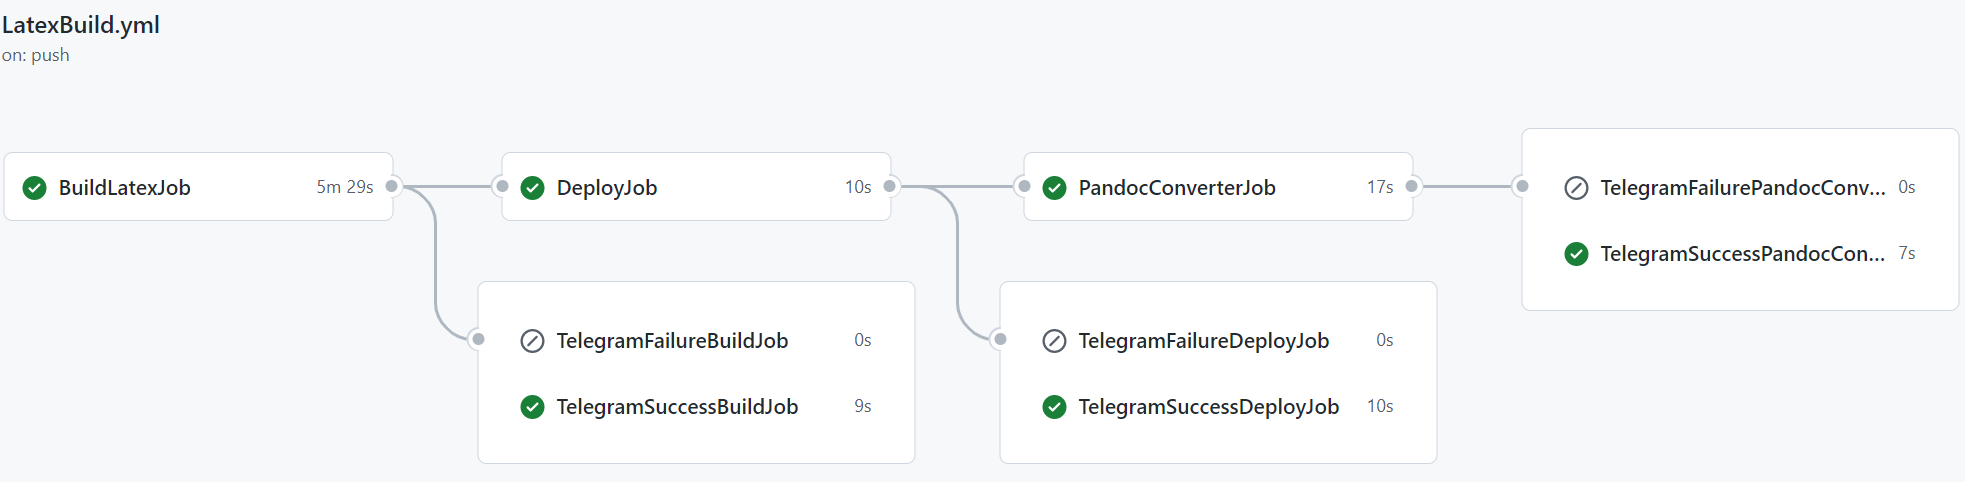
\includegraphics[width=1\textwidth]{Images/gh-pipeline.png}
        \end{figure}

        Qualora una persona volesse consultare la relazione online, senza scaricare il pdf, si è fatto uso di \textbf{Pandoc} per generare il relativo sito web, consultabile comodamente sul browser. Per la paginazione un template html/css è stato utilizzato per rendere la vista più accattivante.

        Il deploy del sito, infine, è stato utilizzato \textbf{GitHub-Pages} che permette di semplificarne la messa in opera avendo un branch dedicato sul quale tutti i file relativi possono essere mantenuti e aggiornati.
        

    \subsection{Progetto}
        \subparagraph{Tool utilizzati}
        \begin{itemize}
            \item Sbt
            \item ScalaTest
            \item GitHub Actions
            \item GitHub Pages
            \item Telegram Bots
            \item Dependabot
            \item Sonarcloud/Codacy/Codefactor
        \end{itemize}
    CI progetto, Test, Coverage, Documentazione, Quality assurance, bla bla
        







